
\subsubsection{Model Generalization}

\begin{figure}[!htb]
    \centering
    \begin{subfigure}[b]{0.49\textwidth}
        \centering
        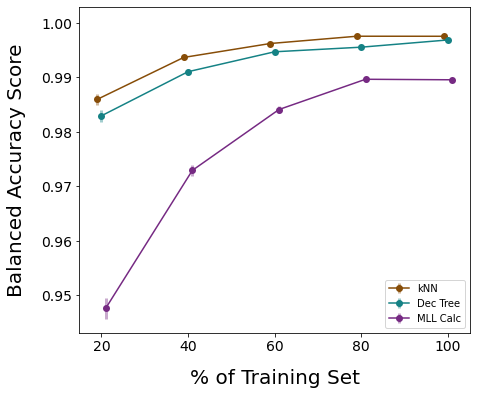
\includegraphics[width=\textwidth]{./chapters/exp1/learncurve_nuc29_BalAcc_rxtr.png}
        \caption{Balanced accuracy of reactor type classification with respect 
                 to training set size.}
        \label{fig:learnsA}
    \end{subfigure}
    \hfill
    \begin{subfigure}[b]{0.49\textwidth}
        \centering
        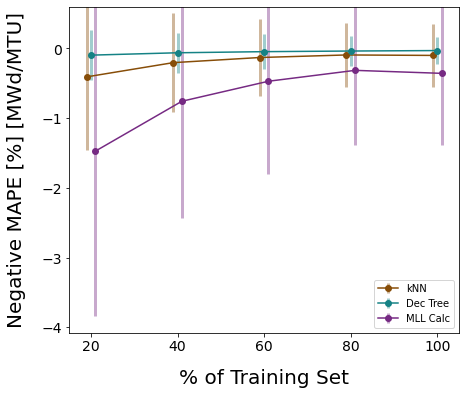
\includegraphics[width=\textwidth]{./chapters/exp1/learncurve_nuc29_MAPE_burn.png}
        \caption{Negative \gls{MAPE} of burnup regression with respect to 
                 to training set size.}
        \label{fig:learnsB}
    \end{subfigure}
    \vskip\baselineskip
    \begin{subfigure}[b]{0.49\textwidth}
        \centering
        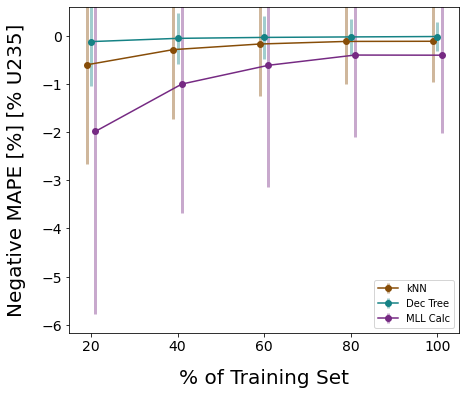
\includegraphics[width=\textwidth]{./chapters/exp1/learncurve_nuc29_MAPE_enri.png}
        \caption{Negative \gls{MAPE} of \gls{U235} enrichment regression with 
                 respect to training set size.}
        \label{fig:learnsC}
    \end{subfigure}
    \hfill
    \begin{subfigure}[b]{0.49\textwidth}
        \centering
        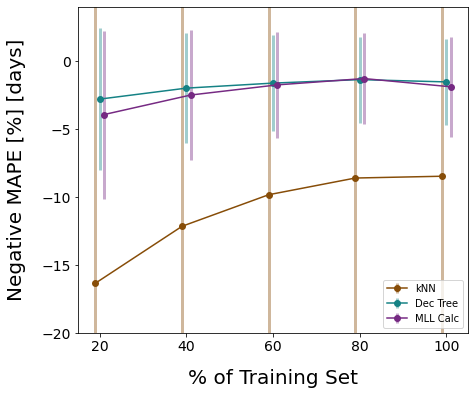
\includegraphics[width=\textwidth]{./chapters/exp1/learncurve_nuc29_MAPE_cool.png}
        \caption{Negative \gls{MAPE} of time since irradiation regression with 
                 respect to training set size.}
        \label{fig:learnsD}
    \end{subfigure}
    \caption{Learning curves for reactor type, burnup, enrichment, and time 
             since irradiation with respect to increasing fraction of the 
             training set.}
    \label{fig:learns}
\end{figure}

Although a key takeaway from Figure \ref{fig:randerr} is that the \gls{MLL}
calculations are the most robust to introduced error in the training set
features for all four prediction categories, there is another aspect of the
algorithm performance not shown in those plots: generalization. \Gls{MLL}
outperforms the scikit-learn methods in part because the training set is so
large. This is because it does not generalize to unseen data; it provides
predictions based on finding the closest training set entry to the test sample.
This is also true for the \textit{k}-nearest neighbor implementations where
$k=1$ (burnup and cooling time, as seen in Table \ref{tbl:exp1hypparam}).

One way to show that an algorithm is generalizing well in comparison to others
is to view the shape of its learning curve (introduced in Section
\ref{sec:complexity}): the prediction performance with respect to training set
size.  Learning curves were constructed for all four prediction categories,
demonstrated in Figure \ref{fig:learns}. As in Figure \ref{fig:randerr}, the
\textit{y}-axis is always oriented so that lower is poorer performance and
higher is better performance; also, the error bars reflect a 99\% confidence
interval for Figure \ref{fig:learnsA}, and one standard deviation of the
average percentage errors for Figures \ref{fig:learnsB}--\ref{fig:learnsD}.
These learning curves represent the 1\% random error case in Figure
\ref{fig:randerr}, so the \gls{MLL} learning curve will be below the
scikit-learn algorithms for the reactor type, burnup, and enrichment
predictions, and the \textit{k}-nearest neighbor learning curve will be below
the \gls{MLL} and decision tree curves for time since irradiation.  Thus, the
scores/errors in Figure \ref{fig:randerr} are the data points at the 100\%
training set level in Figure \ref{fig:learns}.  \todo[inline]{would it be
better to flip the x-axis so that performance degradation travels right as in
the random error plots?}

Figure \ref{fig:learnsA} shows that the balanced accuracy score of reactor type
classification for the \gls{MLL} calculations decreases more at lower training
set size than for the scikit-learn algorithms.  This pattern holds true for the
burnup \gls{MAPE} in Figure \ref{fig:learnsB} and the enrichment \gls{MAPE} in
Figure \ref{fig:learnsC}, although the standard deviation is large enough for
the \gls{MLL} values that the two sets of scikit-learn values are encompassed
by that range. Lastly, Figure \ref{fig:learnsD} has the error bars cropped out
for the \textit{k}-nearest neighbors curve in order to better see the \gls{MLL}
and decision tree curves. The latter two follow a nearly equivalent path, and
the decrease in performance for \textit{k}-nearest neighbors happens mostly in
parallel with them. As with the other regression cases, it is difficult to draw
a conclusion about the trend. While the 20\% and 40\% data points do seem to be
diverging faster, the error bars are too large to state anything definitive.

\subsubsection{Reactor Type Prior Knowledge}

There is similar work being done \todo{get tamu citation} to this that focuses
on these prediction categories but in a serial manner, i.e., first determining
the reactor type before moving forward with other predictions.
\todo[inline]{Finish intro here. Can't get the table to compile yet, so leaving
out for now}

\begin{figure}[!htb]
  \centering
  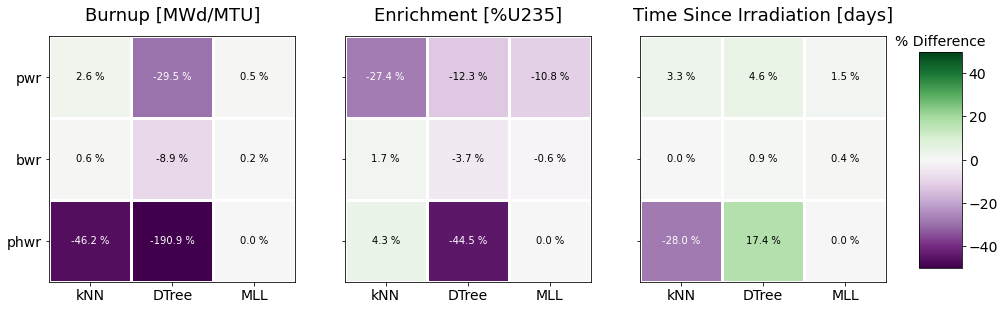
\includegraphics[width=1.1\textwidth]{./chapters/exp1/rxtr-type_known-unknown_diff.png}
  \caption{Heatmaps for the three regression cases showing the percent 
           difference in prediction error between a known reactor type 
           and unknown reactor type.}
  \label{fig:knownrxtr}
\end{figure}

%\begin{table}[!htb]
%  \centering
%  \begin{tabular}{@{}llllllll@{}} \toprule
%    \begin{tabular}[c]{@{}l@{}}Prediction\\ Parameter\end{tabular} 
%     & Reactor Type & kNN Known & kNN Unknown & DTree Known & DTree Unknown & MLL Known & MLL Unknown \\ \toprule
%    \multirow{3}{*}{\begin{tabular}[c]{@{}l@{}}Burnup\\ [MWd/MTU],\\ MAPE\end{tabular}}
%     & PWR & 0.08 & 0.08 & 0.03 & 0.04 & 0.24 & 0.25 \\
%     & BWR  & 0.11  & 0.10  & 0.03 & 0.03 & 0.40 & 0.40 \\
%     & PHWR & 0.13  & 0.19  & 0.01 & 0.03 & 0.29 & 0.29 \\ \midrule
%    \multirow{3}{*}{\begin{tabular}[c]{@{}l@{}}Enrichment\\ [\% U235], \\ MAPE\end{tabular}}
%     & PWR & 0.10 & 0.11 & 0.02 & 0.02 & 0.26 & 0.29 \\
%     & BWR  & 0.12  & 0.12  & 0.02 & 0.02 & 0.46 & 0.46 \\
%     & PHWR & 0.00  & 0.00  & 0.00 & 0.00 & 0.00 & 0.00 \\ \midrule
%    \multirow{3}{*}{\begin{tabular}[c]{@{}l@{}}Time Since \\ Irradiation\\ [days], \\ MAPE\end{tabular}}
%     & PWR & 6.47 & 6.13 & 1.50 & 1.43 & 1.55 & 1.46 \\
%     & BWR  & 9.18  & 9.15  & 1.56 & 1.53 & 2.07 & 2.05 \\
%     & PHWR & 13.78 & 18.62 & 4.51 & 3.71 & 2.30 & 2.30 \\ \bottomrule
%  \end{tabular}
%  \caption{Caption.}
%  \label{tbl:knownrxtr}
%\end{table}

The workflow was repeated for the three regression cases where they were
trained on reactor type-filtered training sets. A 1\% random error was applied
to these training sets, and the 1\% random error full training set was used as
comparison.  Figure \ref{fig:knownrxtr} is three heatmaps that show the percent
difference in prediction \gls{MAE} for each algorithm and reactor type between
the reactor type being known versus unknown prior to prediction. This is
reflected by a diverging color bar as well as a positive or negative percentage
in each square.  The positive percentages indicate the error decreased/improved
from the unknown reactor type case to the known reactor type case.  The
negative percentages indicate the error increased/worsened from the unknown to
the known case. 

For burnup prediction, most differences are within $\pm10\%$ except for three
scenarios.  The decision tree algorithm has improved burnup prediction for
\gls{PWR}s by almost 30\% and for \gls{PHWR}s by almost 200\% given a known
reactor type.  The \textit{k}-nearest neighbors algorithm has 46\% improved
burnup prediction for the \gls{PHWR}. For \gls{U235} enrichment, the \gls{PWR}
predictions all improve by over 10\%, including for the \gls{MLL} algorithm.
This is the only scenario where there is an appreciable difference in \gls{MLL}
performance. The decision tree enrichment prediction of \gls{PHWR}s also has a
sizeable improvement of 44\%.  The time since irradiation predictions for the
most part do not show improvement outside of $\pm10\%$. Of note is some
volatile behavior for the \gls{PHWR} case with the scikit-learn algorithms.
While \textit{k}-nearest neighbors improves by 28\%, the decision tree
predictions were worse by 17\%.

The improvements in the \gls{PHWR} predictions are not surprising since the
generalization of the scikit-learn algorithms could lead to the unique
\gls{PHWR} cases being ignored, since they are after all only 1.5\% of the
training set.  Another interesting result is that the \gls{BWR} predictions
experience no large changes, which makes sense given that they comprise 72\% of
the training set. Also, the \gls{MLL} predictions are approximately the same,
which is expected because this algorithm does not generalize, and the
prediction comes as a set of labels and is therefore already linked to the
reactor type.  The only confounding behavior is the performance decrease in the
\gls{PHWR} enrichment prediction by the decision tree method.  Overall, it is
important to be aware that the regression labels coming from a \gls{PHWR} will
be unlikely to be optimal results (except for those from \gls{MLL}
calculations).

